ATTACHMENT II

ARAKAWA GRIDS

Arakawa grids were first described in Arakawa and Lamb (1977).\footnote{Arakawa, A. and V.R. Lamb, 1977: Computational design of the basic dynamical processes of the UCLA general circulation model. \emph{Methods of Computational Physics} 17\emph{,} New York: Academic Press, pp. 173--265.} There are several different grids with unique staggers labelled as A, B, C, D and E. The following examples show how many of these grids can be defined in GRIB2 using grid definition template 3.1 along with bits 5 through 8 of Flag table 3.4. The relevant bit settings are noted where applicable.

\textbf{\\
}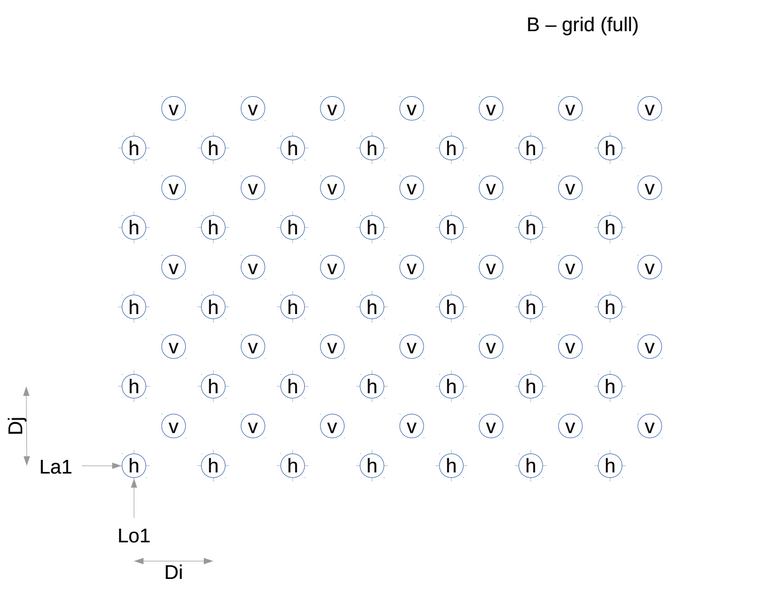
\includegraphics[width=6.49931in,height=5.07361in]{../tex/extracted-media/media/image1.png}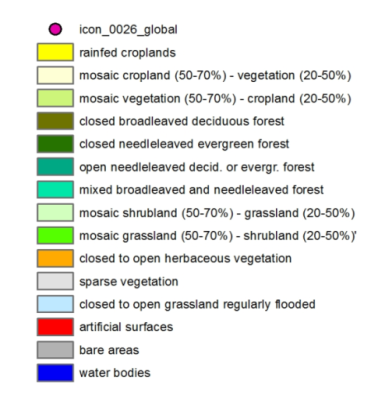
\includegraphics[width=6.49931in,height=4.81528in]{../tex/extracted-media/media/image2.png}\textbf{\\
}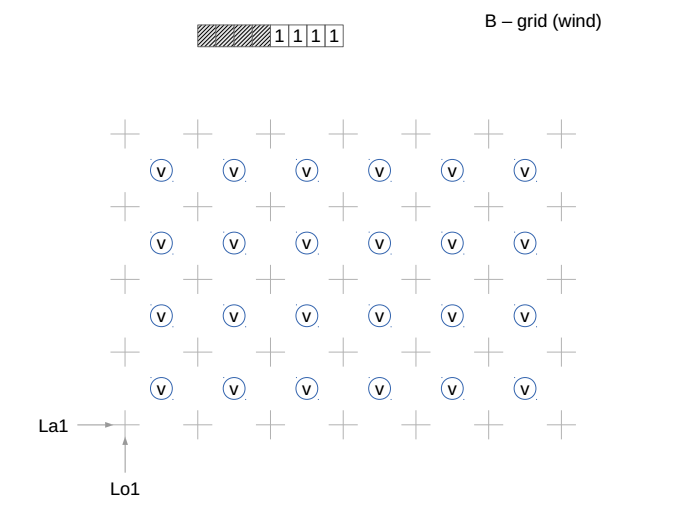
\includegraphics[width=6.49931in,height=4.83611in]{../tex/extracted-media/media/image3.png}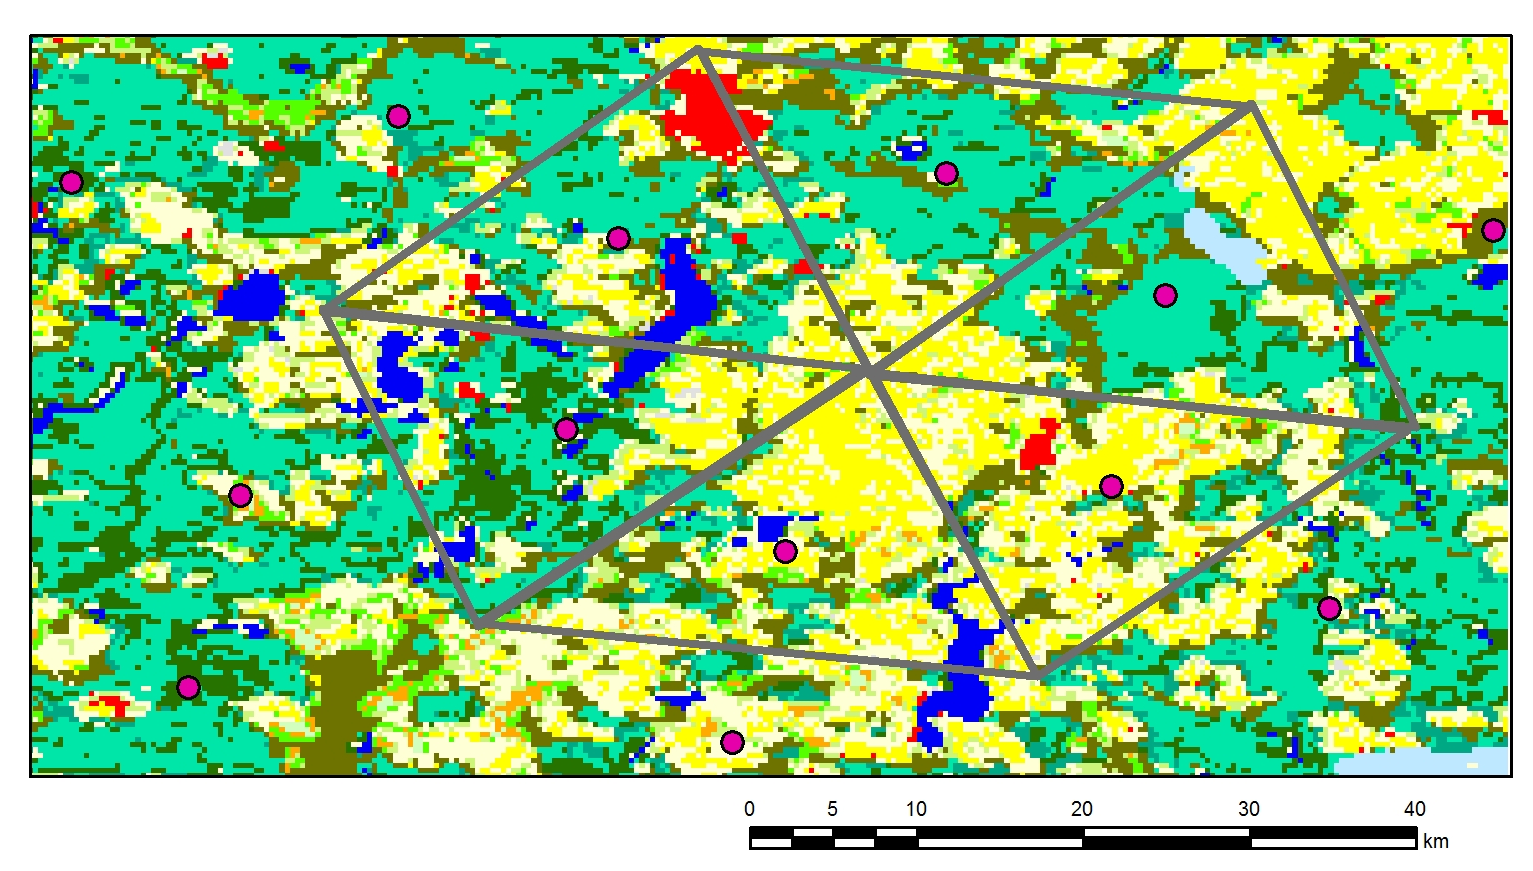
\includegraphics[width=6.49931in,height=4.86111in]{../tex/extracted-media/media/image4.png}\textbf{\\
}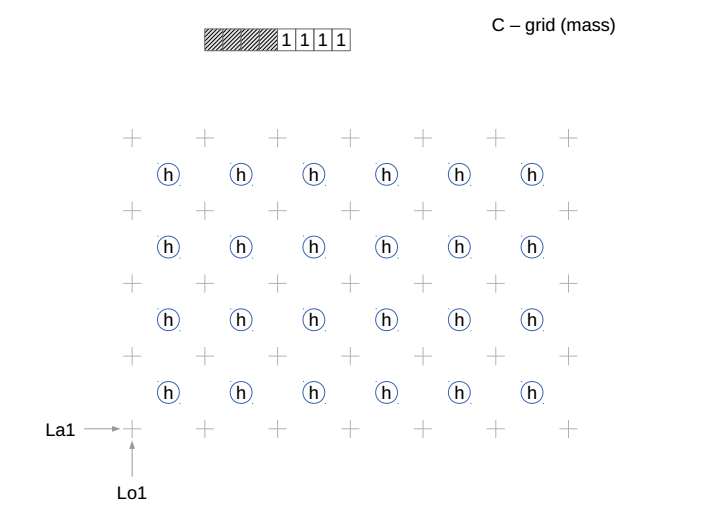
\includegraphics[width=6.49931in,height=4.87153in]{../tex/extracted-media/media/image5.png}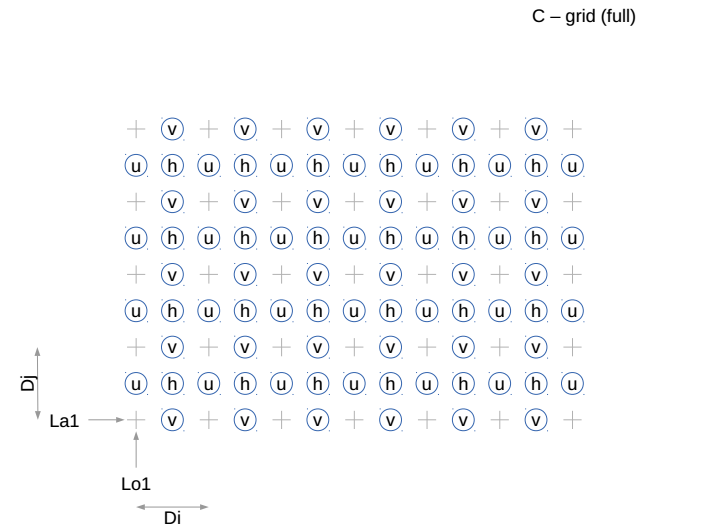
\includegraphics[width=6.49931in,height=4.89306in]{../tex/extracted-media/media/image6.png}\textbf{\\
}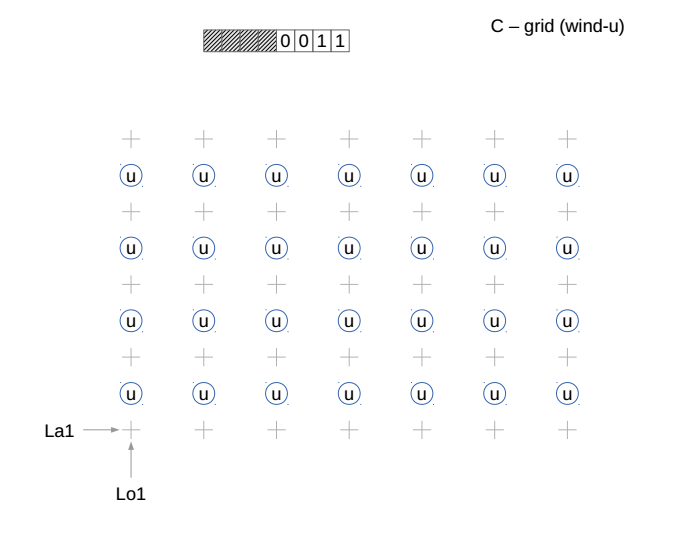
\includegraphics[width=6.49931in,height=5.15694in]{../tex/extracted-media/media/image7.png}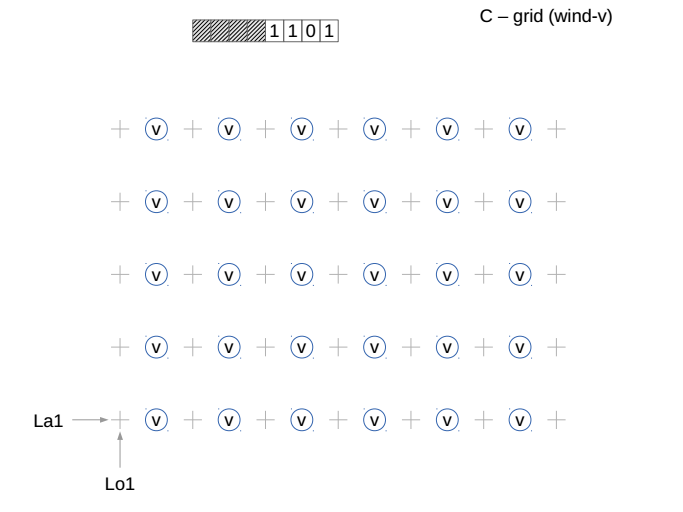
\includegraphics[width=6.49931in,height=4.87153in]{../tex/extracted-media/media/image8.png}\textbf{\\
}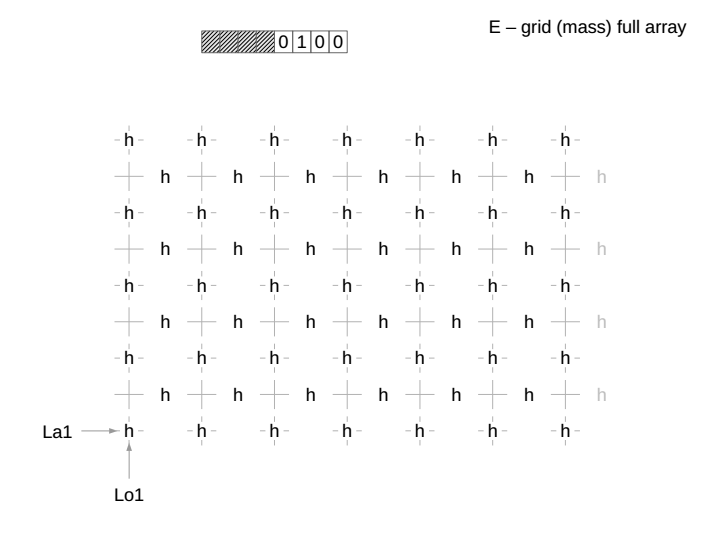
\includegraphics[width=6.49931in,height=4.92361in]{../tex/extracted-media/media/image9.png}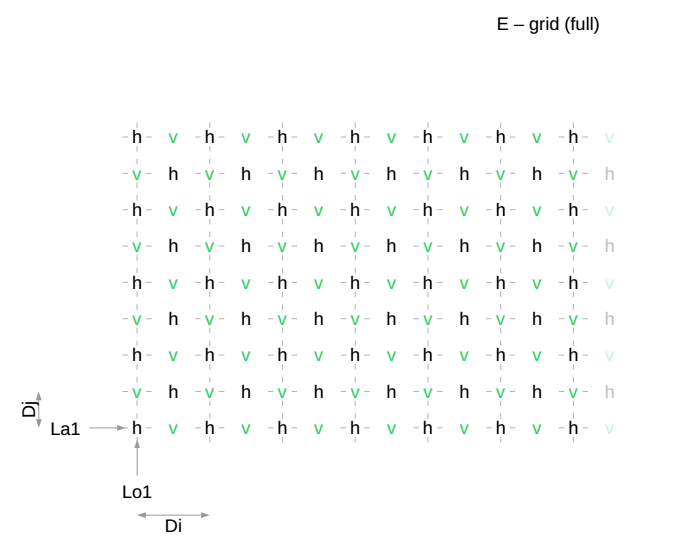
\includegraphics[width=6.49931in,height=5.15972in]{../tex/extracted-media/media/image10.png}\textbf{\\
}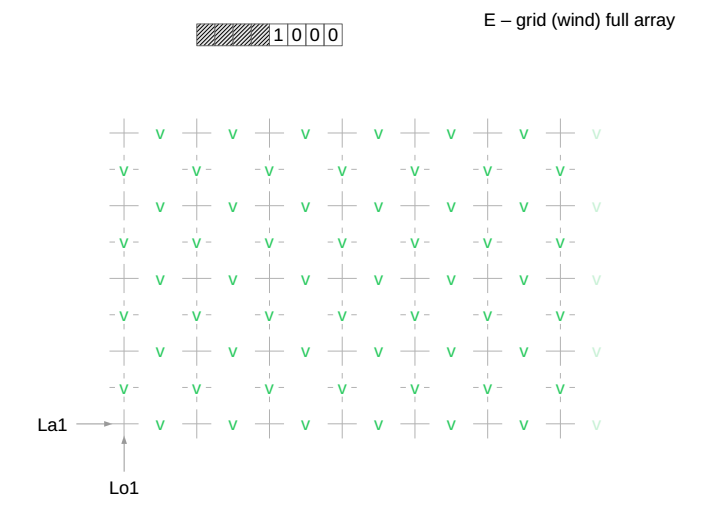
\includegraphics[width=6.49931in,height=4.71042in]{../tex/extracted-media/media/image11.png}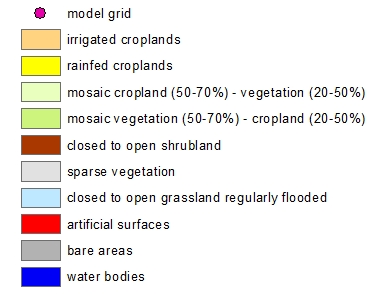
\includegraphics[width=6.49931in,height=4.60764in]{../tex/extracted-media/media/image12.png}\textbf{\\
}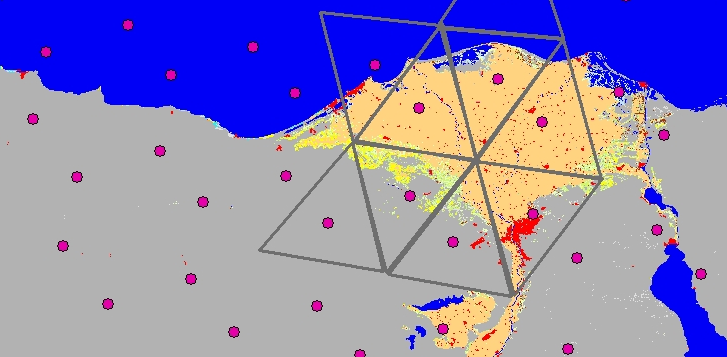
\includegraphics[width=6.49931in,height=4.62639in]{../tex/extracted-media/media/image13.png}
